\documentclass[11pt,a4paper]{article}
\usepackage{fontspec}
\usepackage{xeCJK}
\xeCJKsetup{CJKspace=true}
\setCJKmainfont{Apple SD Gothic Neo}
\setmainfont{Times New Roman}
\usepackage{amsmath,amssymb,bm}
\usepackage{booktabs}
\usepackage{longtable}
\usepackage{graphicx}
\graphicspath{{simulation/}}
\usepackage{geometry}
\geometry{margin=2.3cm}
\usepackage[hidelinks]{hyperref}
\usepackage{caption}
\captionsetup{font=small}

\title{\textbf{Methodology and Empirical Results for L4 Risk-Card Consolidation}\\[4pt]
\large Multi-Resolution Dendrogram, Generative Naming with Two-Reviewer Adjudication, and Source-Corruption Correction (Consolidated Technical Report v2)}
\author{Youngsam Chun (Responsible AI, KT)}
\date{August 6, 2026}

\begin{document}
\maketitle

\begin{abstract}
This report documents the consolidation methodology and empirical results for all 1,660 active L4 risk cards of RAI Risk Taxonomy 2.0 (v2.18.0-rc). The procedure has six stages: (1) build a multi-resolution dendrogram from BGE-M3 embeddings with agglomerative hierarchical clustering; (2) quantify cluster structure, quality, and stability with a threshold sweep over $\tau \in [0.70, 0.94]$; (3) generate draft names and definitions for merged cards at the operational merge level $\tau_{op}=0.88$ using a local generative model; (4) adjudicate the drafts through two independent expert reviewers (terminology/bilingual editing; AI-safety domain); (5) verify the label--definition mismatches surfaced by review against the original source literature and recover the true definitions; and (6) feed the corrections back into the merge decisions. Three findings stand out. First, complete linkage preserves the hierarchy down to $\tau=0.70$ without percolation collapse, whereas single linkage collapses below $\tau \approx 0.78$. Second, as $\tau$ decreases, the noise stability of L3 mapping remains high (agreement $\geq 0.94$) while taxonomic legitimacy decays monotonically (auto rate $0.67 \to 0.22$). Third, two of the eleven embedding-based merge candidates were artifacts of duplicated definitions in the source data; a full screening located exactly three corrupted pairs (six cards, all from the global\_1726 extraction pipeline), and the true definitions were recovered from the original sources. After re-running on the canonical embeddings with a do-not-merge exclusion list, the final adjudication approves 8 of 9 merge groups and rejects 1 as a lexical false positive, for a net reduction of 8 cards this round.
\end{abstract}

\section{Background and Scope}

A prior review showed that the legacy 182-card Physical AI set was already deduplicated at $\tau_{\mathrm{merge}}=0.94$ (maximum pairwise similarity 0.909), so threshold adjustment alone cannot reduce it. The strategy was therefore revised: all 1,660 active L4 cards (General 1,221, Agentic 281, Physical 158) are included, and $\tau$ is lowered stepwise to 0.70. The preliminary analysis established that this descent must be interpreted as multi-resolution hierarchy construction rather than destructive merging; this report records the full empirical program. All outputs are written to a dedicated folder (\texttt{reports/consolidation/simulation/}); the release data is used read-only.

\section{Related Literature}

The merge threshold $\tau$ used throughout this work is best understood at the intersection of four literatures.

\textbf{Hierarchical clustering and cut levels.} In agglomerative hierarchical clustering, $\tau$ corresponds to a dendrogram cut height ($1-\tau$ in cosine distance), and cutting the same dendrogram at several heights yields a multi-resolution view of the data. The choice of linkage criterion is decisive: single linkage is known to suffer from chaining, whereas complete linkage requires all within-group pairs to clear the threshold and therefore produces compact, clique-like groups \cite{murtagh2012}. Our finding that single linkage collapses at $\tau \leq 0.78$ while complete linkage remains stable to $\tau=0.70$ is a direct instance of this classical contrast.

\textbf{Percolation in geometric graphs.} The threshold graph $G_\tau$ over unit-sphere embeddings is a geometric graph, and lowering $\tau$ is equivalent to increasing the connection radius. The theory of random geometric graphs establishes that a giant component emerges sharply at a critical radius \cite{penrose2003}; the empirical onset we observe at $\tau_c \approx 0.78$ under single linkage is the percolation transition that any similarity-threshold merging procedure must stay above. This motivates defining the lower bound of $\tau$ as the maximum of the percolation onset and quality-based thresholds.

\textbf{Cluster validity and stability.} Because no ground-truth partition exists for a risk taxonomy, we rely on internal validity and stability criteria: the silhouette coefficient for cohesion-separation quality \cite{rousseeuw1987}, the Adjusted Rand Index for chance-corrected agreement between partitions \cite{hubert1985}, and perturbation-based stability analysis, which treats a clustering as trustworthy only if it is reproducible under small distortions of the input \cite{vonluxburg2010}. Our observation that two-card merge groups dissolve under $\sigma=0.01$ noise (ARI $\approx 0$) while the coarse levels retain partial stability is exactly the pattern stability theory predicts for structures near the resolution limit of the data, and it grounds our rule that thresholds may nominate merge candidates but only expert adjudication may confirm them.

\textbf{Deduplication and construct validity.} Merging near-duplicate risk cards is an instance of record linkage and entity resolution, for which the classical decision-theoretic formulation already frames the threshold as a trade-off between false merges and missed merges \cite{fellegi1969}; $\tau$ inherits this precision-recall character, so no single value is ``correct'' independent of purpose. Finally, whether two textually similar cards denote the same risk is a question of construct validity in the psychometric sense: statistical association can support but never replace the theoretical judgment that two indicators measure the same construct \cite{cronbach1955}. The explicit-versus-implicit hazard-refusal pair in our data (cosine 0.909, yet distinct benchmark constructs) illustrates why embedding similarity and construct identity must be kept separate. The embedding and keyphrase machinery itself follows the multilingual BGE-M3 encoder \cite{chen2024} and the class-based TF-IDF procedure of BERTopic \cite{grootendorst2022}.

\section{Methodology}

\subsection{Embedding and Dendrogram Construction}

Each card's bilingual text $x_i = \mathrm{label}^{en}_i \| \mathrm{label}^{ko}_i \| \mathrm{def}^{en}_i \| \mathrm{def}^{ko}_i$ is encoded with BGE-M3 (ollama implementation) to $\mathbf{e}_i \in \mathbb{S}^{1023}$. Agglomerative clustering is run on pairwise cosine distance $d_{ij}=1-\mathbf{e}_i\cdot\mathbf{e}_j$ under complete, average, and single linkage. The complete-linkage merge condition, $\min_{i,j\in C} s_{ij} \geq \tau$, structurally blocks chaining.

\subsection{Threshold Sweep and Reliability Metrics}

The cut level $\tau$ is lowered from $0.94$ to $0.70$ in steps of $\Delta\tau=0.02$ while four metrics are tracked: the auto rate (fraction of merge groups whose members share a single existing L3 that coincides with the re-mapped L3), the mean margin $s_{(1)}-s_{(2)}$, the perturbation agreement of L3 mapping (Gaussian noise $\sigma=0.01$, 50 repeats), and the silhouette coefficient. Cluster-structure stability is measured separately with the Adjusted Rand Index (ARI; $\sigma\in\{0.01,0.03,0.05\}$, 30 repeats).

\subsection{New-Card Generation and Two-Reviewer Adjudication}

For multi-card groups at $\tau_{op}=0.88$, draft bilingual names and definitions are generated from c-TF-IDF top terms and a local generative model (qwen3:4b). Because generative drafts cannot be trusted, two independent reviewers examine them post hoc: Reviewer A handles terminology and bilingual editing (mistranslation fixes, register), Reviewer B handles AI-safety domain validity (construct validity of the merge, L3 mapping, source-corruption detection). The two opinions are consolidated into approved or defer. The L3 re-mapping of each new card uses nearest-centroid assignment $\hat{k}=\arg\max_k \bar{\mathbf{e}}_C\cdot\boldsymbol{\mu}_k$ and is validated with the three checks from the main technical report (EM convergence, top-k containment, perturbation stability).

\subsection{Source-Corruption Verification}

For the label--definition mismatches flagged by Reviewer B, (i) all 1,660 active cards are screened for the identical-definition/different-label pattern, and (ii) the referenced source documents (arXiv HTML, government report PDF) are checked directly to recover the true definitions.

\section{Empirical Results}

\subsection{Structure: the Linkage Rule Determines the Outcome}

\begin{table}[htbp]
\centering
\caption{Cluster structure by cut level (complete vs single linkage)}
\begin{tabular}{cccccc}
\toprule
$\tau$ & \multicolumn{3}{c}{complete linkage} & \multicolumn{2}{c}{single linkage} \\
\cmidrule(lr){2-4}\cmidrule(lr){5-6}
 & clusters & largest & cross-L1 & clusters & largest \\
\midrule
0.94 & 1,660 & 1 & 0 & 1,659 & 2 \\
0.88 & 1,649 & 2 & 1 & 1,635 & 2 \\
0.82 & 1,553 & 3 & 11 & 1,463 & 8 \\
0.76 & 1,254 & 5 & 62 & 1,000 & 513 \\
0.70 & 873 & 9 & 114 & 490 & 1,470 \\
\bottomrule
\end{tabular}
\end{table}

Under single linkage the giant component exceeds 5\% of the corpus at $\tau=0.78$ and reaches 89\% at 0.70, a clear percolation collapse. Complete linkage remains stable (largest cluster 9 at $\tau=0.70$), and the coarse thematic clusters it produces (AI overreliance, 9 cards; loss of control, 7; opacity/transparency, 6) are meaningful candidates for a data-driven upper structure.

\begin{figure}[htbp]
\centering
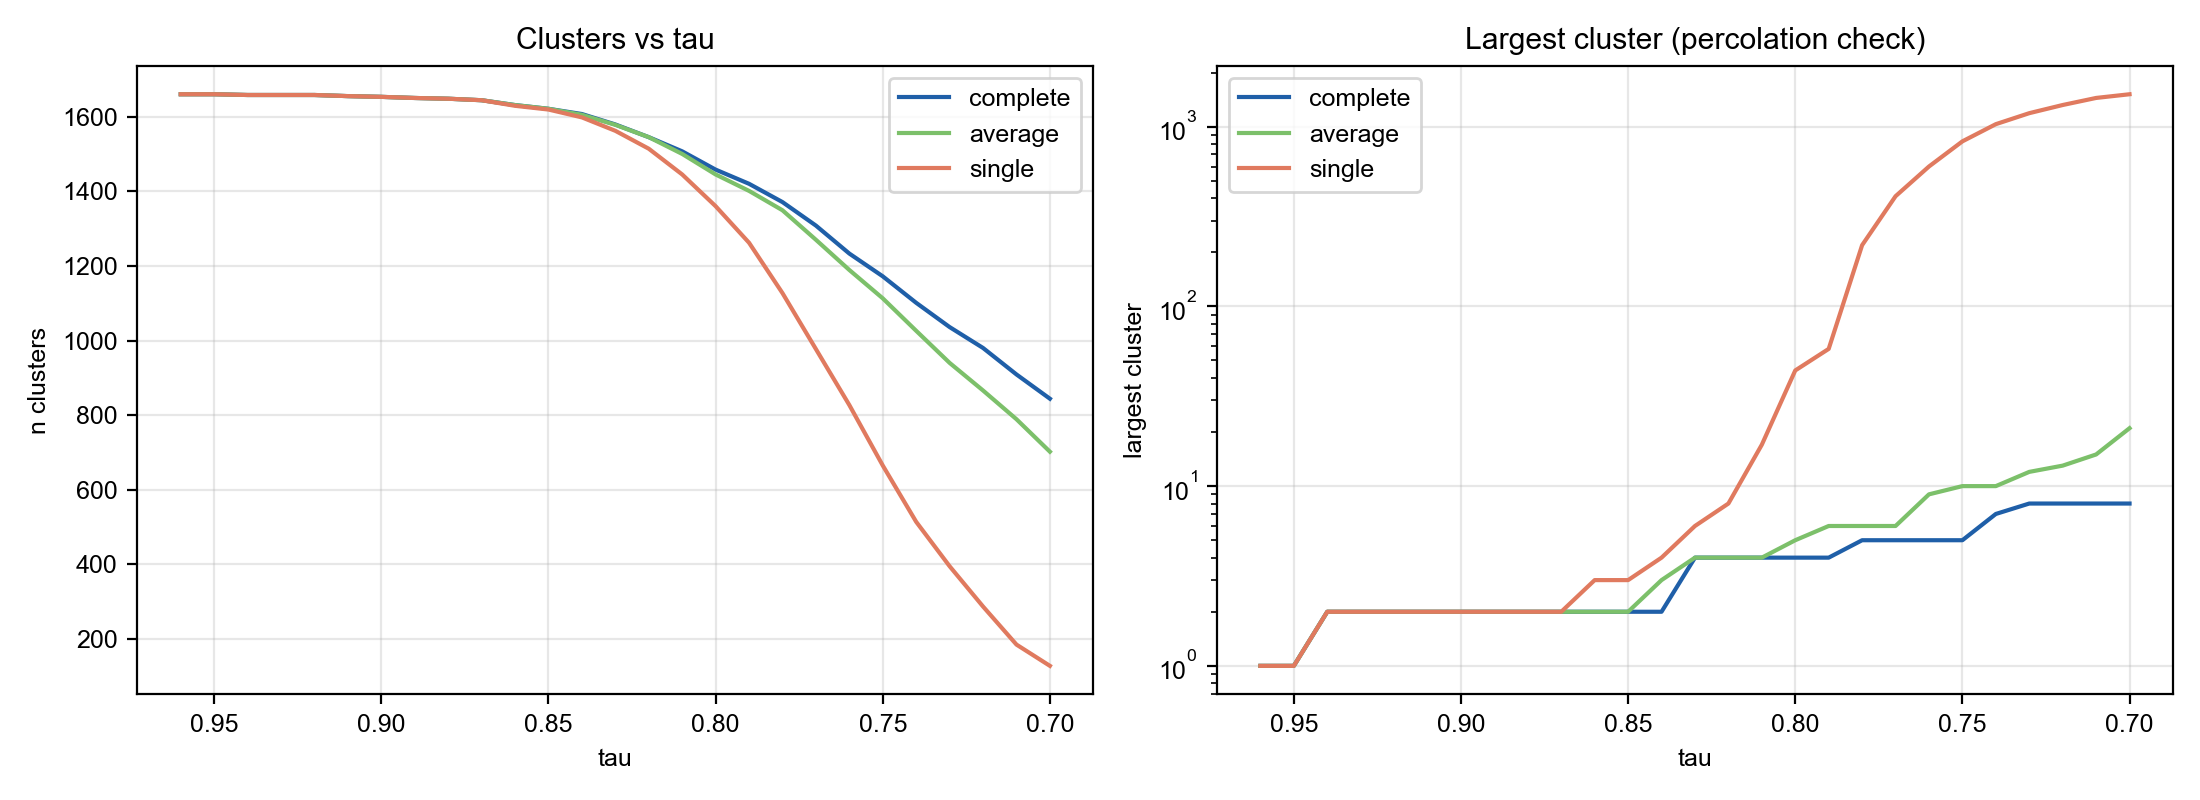
\includegraphics[width=0.95\linewidth]{fig_merge_curve.png}
\caption{Reduction curve (left) and largest-cluster size (right, log scale). The percolation collapse of single linkage is evident.}
\end{figure}

\subsection{The Duality of Reliability as $\tau$ Decreases}

\begin{figure}[htbp]
\centering
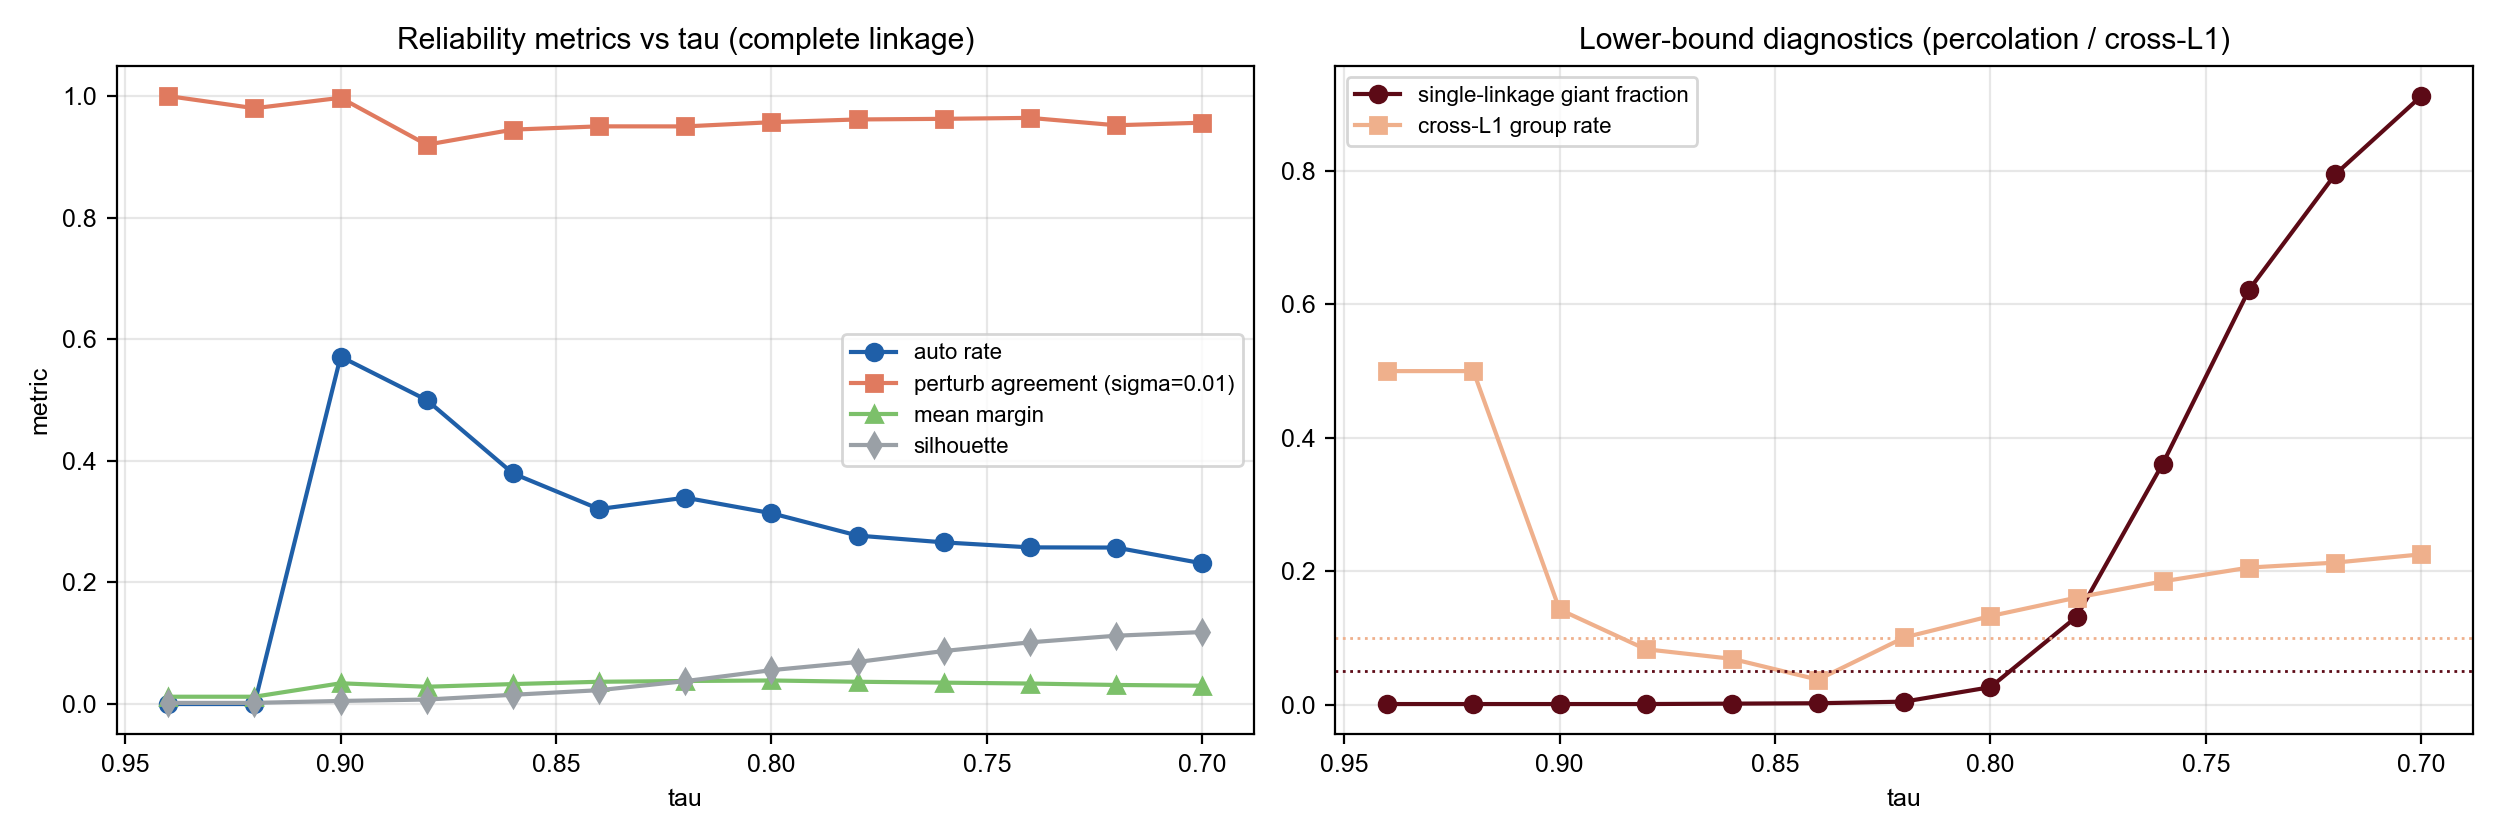
\includegraphics[width=0.95\linewidth]{fig_tau_reliability_sweep.png}
\caption{Reliability metrics over the $\tau$ sweep (left) and lower-bound diagnostics (right).}
\end{figure}

Perturbation agreement stays within $0.94 \sim 0.98$ across the whole range, but the auto rate falls monotonically from $0.67$ ($\tau=0.90$) to $0.22$ ($\tau=0.70$) and the cross-L1 contamination rate rises to 0.23. Mechanical mapping stability and taxonomic legitimacy therefore decouple, and the cost of lowering $\tau$ falls entirely on the latter. Cluster-structure ARI collapses to near zero at the fine level ($\tau=0.88$) even under $\sigma=0.01$, showing that two-card merge groups are fragile to embedding perturbations. This is the quantitative basis for prohibiting threshold-only merge confirmation and requiring expert adjudication.

The lower bound for $\tau$ is defined as the maximum of three thresholds: the single-linkage percolation onset ($\tau_c \approx 0.78$), the 10\% cross-L1 contamination threshold, and the 90\% agreement threshold. Empirically the operational merge floor is $0.88 \sim 0.90$, the display-hierarchy floor is $0.78$, and the recommended step is $\Delta\tau=0.02$ (refined to 0.01 near the floor).

\subsection{Reliability of the New-Card to L3 Mapping}

Applying the three checks to the eleven merge groups at $\tau_{op}=0.88$: EM converges in 2 steps ($J: 0.831 \to 0.845$), top-1/top-3 containment is 100\%, and perturbation stability is 96.0\% at $\sigma=0.01$ and 83.9\% at $\sigma=0.05$ (200 repeats). The mapping itself is trustworthy, but margins are thin for some groups ($0.002 \sim 0.094$), warranting per-group inspection.

\begin{figure}[htbp]
\centering
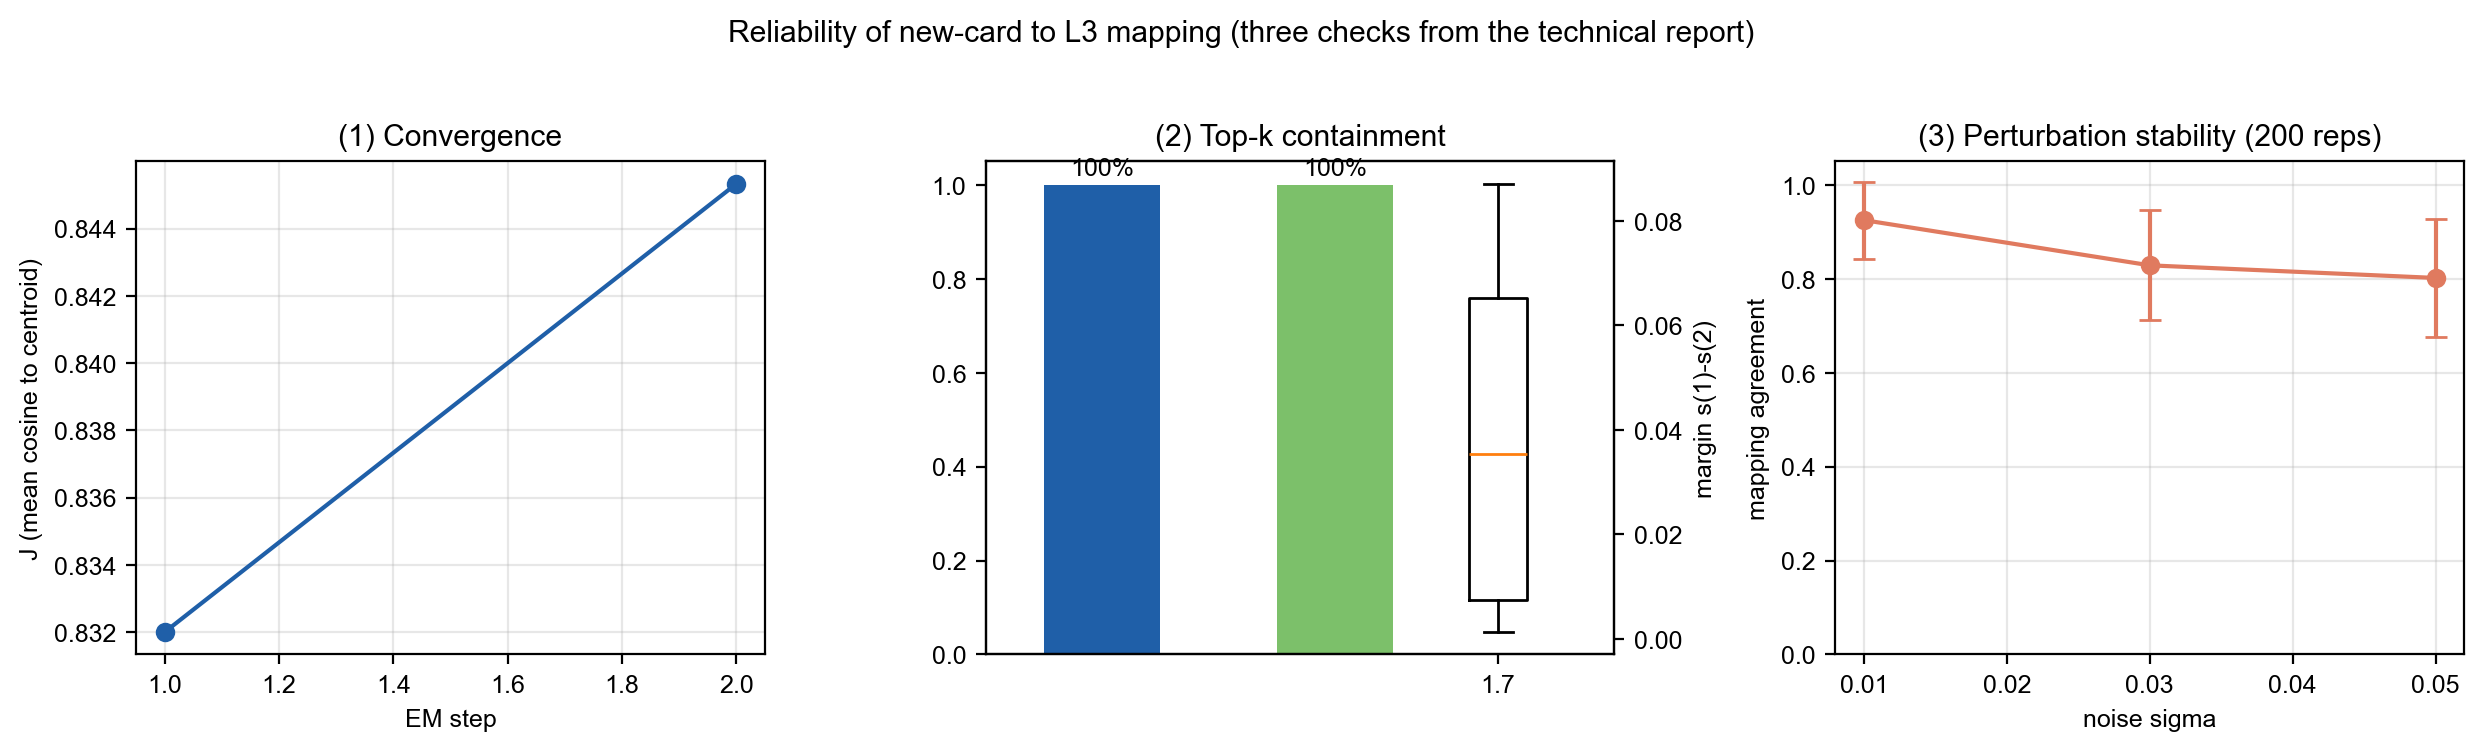
\includegraphics[width=0.95\linewidth]{fig_l3_mapping_reliability.png}
\caption{Three reliability checks for the new-card to L3 mapping: (1) EM convergence, (2) top-k containment and margin, (3) perturbation stability.}
\end{figure}

\subsection{Two-Reviewer Adjudication and the Discovery of Source Corruption}

Of the eleven drafts, Reviewer A supplied terminology and register corrections throughout (e.g., replacing a mistranslation of \emph{contestability}, and of \emph{frontier AI}, in the Korean labels), while Reviewer B deferred four groups. The deferral reasons were: label--definition mismatch inside member cards (g1462, g1458), over-merging of two distinct benchmark constructs (explicit vs implicit hazard refusal, g81), and mechanism mixing plus an L3 misassignment (g1582). Reviewer B additionally identified three disinformation cards in the same L3 (g520, g1388, g1389) as substantive duplicates, designated for umbrella consolidation in the next round.

\subsection{Full Screening and Correction of Source Corruption}

The full screening found exactly three corrupted pairs (six cards), all from the global\_1726 source with the \texttt{source\_mechanism\_only\_v2.7} extraction pipeline. Direct comparison against the original sources yielded the following.

\begin{table}[htbp]
\centering
\small
\caption{Diagnosis and correction of the three source-corruption cases}
\begin{tabular}{p{2.7cm}p{3.3cm}p{3.1cm}p{5.1cm}}
\toprule
Cards & Corruption type & Original source & Correction and feedback into merge decisions \\
\midrule
RAI4-0659 (mass disinformation generation) & Definition mis-copied from RAI4-0892 (alternative financial data) & Gipi\v{s}kis et al., arXiv:2410.23472 (GPAI risk catalog) & True definition recovered. Merge g1462 void. 0659 joins the disinformation umbrella; 0892 remains a standalone financial-data card \\
RAI4-0863 (AI advice influencing moral judgment) & Definition mis-copied from RAI4-0870 (GPAI agents in finance) & arXiv:2410.23472, \S10.3 & True definition recovered. Merge g1458 void. 0863 split off and re-mapped to a values/interaction L3; 0870 stays under RAI3-A-SYS-05 \\
RAI4-1427/1428 (bias amplification / harmful responses) & Over-splitting of a single source sentence & UK Government Office for Science (2023), \emph{Future Risks of Frontier AI}, Annex A \S79 & The source is a single risk statement, so merge g1582 is justified (overturning Reviewer B's split recommendation on source evidence); the L3 is re-mapped from the Agentic to the General branch \\
\bottomrule
\end{tabular}
\end{table}

These results show that some embedding-similarity merge candidates are artifacts of upstream data-quality defects, and conversely that the merge pipeline doubles as a data-quality audit.

\subsection{Final Adjudication (Canonical-Embedding Round)}

The pipeline was then re-run on the canonical embeddings with the confirmed exclusions applied as a do-not-merge list (the explicit/implicit hazard-refusal pair and the two corruption-artifact pairs). This produced 9 merge groups. Seven carried over from the first round and retained their adjudications; two were new. The new pair of agent tool-misuse cards (RAI4-0479, RAI4-1669) was approved by both reviewers as a single construct, with the caveat that its HOLD placement must be resolved to a real agentic L3 before finalization. The new violent/non-violent crime pair (RAI4-0682, RAI4-0691; cosine 0.945) was rejected: the similarity is a lexical artifact of the shared ``crimes'' anchor, established content-safety taxonomies (MLCommons AILuminate, Llama Guard) deliberately keep the two apart, and the pair is now registered as a known embedding false positive in the do-not-merge list. The corruption-justified merge of the bias-amplification pair (RAI4-1427/1428) was approved on source evidence with a General-branch L3 re-map.

The final tally is therefore 8 merges approved, 1 rejected, 0 pending, for a net reduction of 8 cards this round. One item remains under review (whether RAI4-1201 is a fraud construct), and the disinformation umbrella consolidation (3--4 further cards) and the resolution of 614 HOLD cards are carried to the next round.

\section{Operating Rules and Open Decisions}

The rules fixed by this study are: (1) merging uses complete linkage only; (2) operational merges (card deletion) are restricted to same-L3 groups at $\tau \geq 0.88$, with thresholds serving only for candidate discovery and confirmation always requiring two-reviewer adjudication; (3) levels at $\tau \leq 0.82$ are used only as display/navigation hierarchy; (4) source integrity (label--definition consistency) of member cards is checked before any merge is confirmed; and (5) every merge ships only through a dated release with \texttt{merged\_into} lineage and a full old-to-new ID mapping.

Open decisions: (i) fixing the canonical embedding pipeline (the ollama implementation and the website proximity network yield 11 vs 91 merge groups at $\tau=0.88$); (ii) the design of the disinformation umbrella card; (iii) the adjudication scheme for the HOLD-resolution round; and (iv) the new-card ID scheme for the v2.19 release.

\section*{Artifact Inventory}

Under \texttt{reports/consolidation/simulation/}: dendrogram\_simulation\_1660.\{ipynb, html\} (Task 1--10 execution record), embeddings\_bge-m3\_1660.npy, level\_assignments\_complete.csv, dendrogram\_summary.json, merged\_card\_proposals\_tau088.csv, draft\_cards\_for\_review.json, reviewed\_cards\_final.json, merge\_before\_after\_reviewed\_tau088.html (three-stage Before/Draft/Reviewed report), source\_corruption\_\{screening, corrections\}.json, and six PNG figures.

\begin{thebibliography}{9}
\bibitem{murtagh2012} Murtagh, F., Contreras, P. (2012). Algorithms for hierarchical clustering: an overview. \emph{WIREs Data Mining and Knowledge Discovery}, 2(1), 86--97. \url{https://doi.org/10.1002/widm.53}
\bibitem{penrose2003} Penrose, M. (2003). \emph{Random Geometric Graphs}. Oxford University Press. \url{https://academic.oup.com/book/9064}
\bibitem{rousseeuw1987} Rousseeuw, P. J. (1987). Silhouettes: a graphical aid to the interpretation and validation of cluster analysis. \emph{Journal of Computational and Applied Mathematics}, 20, 53--65. \url{https://doi.org/10.1016/0377-0427(87)90125-7}
\bibitem{hubert1985} Hubert, L., Arabie, P. (1985). Comparing partitions. \emph{Journal of Classification}, 2, 193--218. \url{https://doi.org/10.1007/BF01908075}
\bibitem{vonluxburg2010} von Luxburg, U. (2010). Clustering stability: an overview. \emph{Foundations and Trends in Machine Learning}, 2(3), 235--274. \url{https://doi.org/10.1561/2200000008}
\bibitem{fellegi1969} Fellegi, I. P., Sunter, A. B. (1969). A theory for record linkage. \emph{Journal of the American Statistical Association}, 64(328), 1183--1210. \url{https://doi.org/10.1080/01621459.1969.10501049}
\bibitem{cronbach1955} Cronbach, L. J., Meehl, P. E. (1955). Construct validity in psychological tests. \emph{Psychological Bulletin}, 52(4), 281--302. \url{https://doi.org/10.1037/h0040957}
\bibitem{chen2024} Chen, J., Xiao, S., Zhang, P., Luo, K., Lian, D., Liu, Z. (2024). BGE M3-Embedding: Multi-lingual, multi-functionality, multi-granularity text embeddings through self-knowledge distillation. arXiv:2402.03216. \url{https://arxiv.org/abs/2402.03216}
\bibitem{grootendorst2022} Grootendorst, M. (2022). BERTopic: Neural topic modeling with a class-based TF-IDF procedure. arXiv:2203.05794. \url{https://arxiv.org/abs/2203.05794}
\end{thebibliography}

\appendix
\section{Appendix: Change Log by Merge Group}

The table below reproduces, per merge group, the actual changes recorded in the reviewed three-stage HTML report (\texttt{merge\_before\_after\_reviewed\_tau088.html}): the member cards (Before), the generative draft, the reviewer-confirmed English label with Reviewer B's decision note, and the final verdict.

\begin{longtable}{p{0.6cm}p{4.2cm}p{3.3cm}p{4.6cm}p{1.5cm}}
\caption{Actual change log per merge group, canonical-embedding round (from the reviewed before/draft/reviewed HTML report)}\\
\toprule
G & Before (member cards) & Draft (qwen3:4b) & Reviewed (final EN label / decision note) & Verdict \\
\midrule\endfirsthead
\toprule G & Before & Draft & Reviewed & Verdict \\ \midrule\endhead
532 & \texttt{RAI4-0124} AI 중재 의사결정 경쟁성 손실\newline \texttt{RAI4-0453} 경쟁성 상실 & AI-mediated decision contestability loss & Loss of contestability in AI-mediated decisions\newline \emph{구제수단 부재와 실질적 접근불가(불투명성·비용) 모두 포괄} & approved \\ \addlinespace
1425 & \texttt{RAI4-0148} AI 동반자 정서적 의존\newline \texttt{RAI4-0454} AI에 대한 정서적 의존성 & Emotional dependence on AI companions and assistants & Emotional dependence on AI companions and assistants\newline \emph{멤버 HOLD 해소 전까지 HOLD 플래그 승계} & approved \\ \addlinespace
582 & \texttt{RAI4-0479} 에이전트 도구 오용\newline \texttt{RAI4-1669} 도구 오용/안전하지 않은 도구 호출 & Agent tool misuse & Agent tool misuse\newline \emph{동일 구성개념(메커니즘·완화책 동일). 단 HOLD는 종착지가 아니므로 확정 전 실제 agentic L3로 해소 필요.} & approved \\ \addlinespace
900 & \texttt{RAI4-0682} 비폭력 범죄\newline \texttt{RAI4-0691} 폭력 범죄 & Responses that enable or encourage nonviolent and violent cr & (merge rejected) keep violent and nonviolent crime cards separate\newline \emph{높은 유사도는 'crimes' 어휘 anchor의 인공물. MLCommons AILuminate·Llama Guard 등 표준 분류가 폭력/비폭력을 분리하며 심각도·완화 정책이 다름. 병합 기각, } & rejected \\ \addlinespace
221 & \texttt{RAI4-0732} 프롬프트의 기밀 데이터\newline \texttt{RAI4-0750} 프롬프트에 개인 정보 & Sensitive information in prompt & Sensitive data included in prompts\newline \emph{964(학습데이터 유출)와 경계 명시, 0750 HOLD 해소} & approved \\ \addlinespace
107 & \texttt{RAI4-0738} 개인정보 노출\newline \texttt{RAI4-0749} 데이터의 개인정보 & Exposure of personal information in model training and fine- & Personal information exposure from training and input data\newline \emph{957(프롬프트 입력)과 경계 명시} & approved \\ \addlinespace
1574 & \texttt{RAI4-1201} AI가 만든 사기\newline \texttt{RAI4-1202} 허위정보 생성 & AI-Generated Malicious Content & Disinformation and harmful content via generative AI\newline \emph{RAI4-1201이 사기(fraud) 구성개념이면 분리, 아니면 520과 통합} & approved \\ \addlinespace
1575 & \texttt{RAI4-1360} 잘못된 정보와 허위 정보\newline \texttt{RAI4-1597} 허위 정보 확산 & Intentional Disinformation Spread via Generative AI & Generative AI-driven disinformation spread\newline \emph{생성 vs 확산 구분 유지 후 520과 차기 통합} & approved \\ \addlinespace
1561 & \texttt{RAI4-1427} 편견의 증폭\newline \texttt{RAI4-1428} 유해한 반응 & Amplification of Biases Leading to Harmful Responses & Bias amplification and harmful responses in frontier AI models\newline \emph{원소스(UK Gov Annex A para 79)가 단일 리스크 서술임을 확인하여 분리 의견 번복. L3는 Agentic이 아닌 General 브랜치로 재매핑 필요.} & approved \\ \addlinespace
\bottomrule
\end{longtable}

\end{document}
